\documentclass[oneside,reqno]{amsart}
\setlength{\textwidth}{\paperwidth}\addtolength{\textwidth}{-2in}\calclayout
\usepackage{amsmath,amsthm}
\usepackage{dsfont} 
\usepackage{tikz}
\usepackage{enumitem}

\DeclareMathOperator{\E}{\mathrm{E}}
\DeclareMathOperator{\var}{\mathrm{var}}
\DeclareMathOperator{\cov}{\mathrm{cov}}
\newcommand{\eps}{\varepsilon}
\newcommand{\Ncal}{\mathcal{N}}
\newcommand{\Ucal}{\mathcal{U}}
\newcommand{\Z}{\mathds{Z}}
\newcommand{\R}{\mathds{R}}
\newcommand{\N}{\mathds{N}}

\theoremstyle{definition}
\newtheorem{prob}{Problem}
\renewcommand*{\proofname}{Solution}
\setlist[enumerate]{label={(\roman*)}}

\title{STAT 433: Homework 3}
\author{Daniel Pfeffer}
\date{\today}
%------------------------------------------------------------------------------
\begin{document}
\maketitle


\begin{prob}
Consider the following transition matrices. Identify the transient and recurrent states, and the irreducible closed sets in the Markov chains.
\end{prob}

\begin{enumerate}
\item 
???
\begin{proof}
The directed graph representation is
\begin{center}
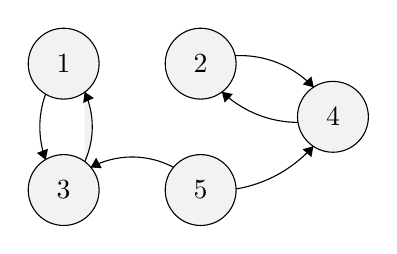
\begin{tikzpicture}[scale=0.15]
\tikzstyle{every node}+=[inner sep=0pt]
\draw [black,fill=gray!10] (21.3,-16.8) circle (3);
\draw (21.3,-16.8) node {$1$};
\draw [black,fill=gray!10] (32.9,-16.8) circle (3);
\draw (32.9,-16.8) node {$2$};
\draw [black,fill=gray!10] (32.9,-27.5) circle (3);
\draw (32.9,-27.5) node {$5$};
\draw [black,fill=gray!10] (21.3,-27.5) circle (3);
\draw (21.3,-27.5) node {$3$};
\draw [black,fill=gray!10] (44.1,-21.3) circle (3);
\draw (44.1,-21.3) node {$4$};
\draw [black,fill=gray!10] (23.077,-19.19) arc (24.56337:-24.56337:7.121);
\fill [black] (23.08,-19.19) -- (22.95,-20.13) -- (23.86,-19.71);
\draw [black] (19.776,-24.936) arc (-159.87842:-200.12158:8.099);
\fill [black] (19.78,-24.94) -- (19.97,-24.01) -- (19.03,-24.36);
\draw [black] (35.807,-16.126) arc (92.97926:43.24163:8.533);
\fill [black] (42.47,-18.8) -- (42.28,-17.88) -- (41.55,-18.56);
\draw [black] (41.151,-21.773) arc (-90.07169:-133.70742:9.35);
\fill [black] (34.7,-19.18) -- (34.93,-20.1) -- (35.63,-19.37);
\draw [black] (42.437,-23.786) arc (-41.47534:-80.58934:11.178);
\fill [black] (42.44,-23.79) -- (41.53,-24.05) -- (42.28,-24.72);
\draw [black] (23.585,-25.587) arc (118.33304:61.66696:7.407);
\fill [black] (23.58,-25.59) -- (24.53,-25.65) -- (24.05,-24.77);
\end{tikzpicture}
\end{center}
Since $1 \to 2$ but $2 \not\to 1$, state 1 is transient. Since $5 \to 4$ but $4 \not\to 5$, state 5 is transient. Since $3 \to 2$ but $2 \not\to 3$, state 3 is transient. So, states 2 and 4 are recurrent. The closed irreducible set is $\{2,4\}$. 
\end{proof}

\item
???
\begin{proof}
The directed graph representation is
\begin{center}
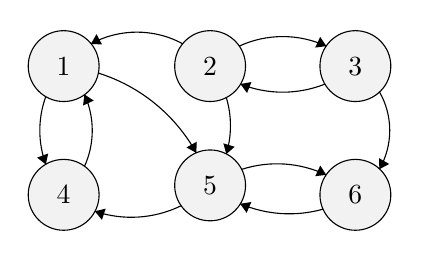
\begin{tikzpicture}[scale=0.15]
\tikzstyle{every node}+=[inner sep=0pt]
\draw [black,fill=gray!10] (20.5,-16.8) circle (3);
\draw (20.5,-16.8) node {$1$};
\draw [black,fill=gray!10] (32.9,-16.8) circle (3);
\draw (32.9,-16.8) node {$2$};
\draw [black,fill=gray!10] (32.9,-26.9) circle (3);
\draw (32.9,-26.9) node {$5$};
\draw [black,fill=gray!10] (20.5,-27.7) circle (3);
\draw (20.5,-27.7) node {$4$};
\draw [black,fill=gray!10] (45.2,-16.8) circle (3);
\draw (45.2,-16.8) node {$3$};
\draw [black,fill=gray!10] (45.2,-27.7) circle (3);
\draw (45.2,-27.7) node {$6$};
\draw [black] (22.26,-19.204) arc (24.50554:-24.50554:7.344);
\fill [black] (22.26,-19.2) -- (22.14,-20.14) -- (23.05,-19.72);
\draw [black] (18.991,-25.126) arc (-159.89496:-200.10504:8.366);
\fill [black] (18.99,-25.13) -- (19.19,-24.2) -- (18.25,-24.55);
\draw [black] (35.36,-15.109) arc (114.74956:65.25044:8.813);
\fill [black] (42.74,-15.11) -- (42.22,-14.32) -- (41.8,-15.23);
\draw [black] (42.629,-18.322) arc (-68.27144:-111.72856:9.667);
\fill [black] (35.47,-18.32) -- (36.03,-19.08) -- (36.4,-18.15);
\draw [black] (30.456,-28.619) arc (-63.84781:-108.76942:9.589);
\fill [black] (23.14,-29.09) -- (23.74,-29.82) -- (24.06,-28.87);
\draw [black] (23.435,-17.392) arc (72.62813:29.04513:14.402);
\fill [black] (31.73,-24.15) -- (31.77,-23.2) -- (30.9,-23.69);
\draw [black] (22.812,-14.915) arc (118.60249:61.39751:8.121);
\fill [black] (22.81,-14.92) -- (23.75,-14.97) -- (23.28,-14.09);
\draw [black] (47.231,-18.972) arc (29.98384:-29.98384:6.559);
\fill [black] (47.23,-25.53) -- (48.06,-25.09) -- (47.2,-24.59);
\draw [black] (34.267,-19.452) arc (16.8627:-16.8627:8.266);
\fill [black] (34.27,-24.25) -- (34.98,-23.63) -- (34.02,-23.34);
\draw [black] (35.565,-25.548) arc (108.03249:64.52488:9.691);
\fill [black] (42.73,-26.01) -- (42.23,-25.22) -- (41.8,-26.12);
\draw [black] (42.467,-28.912) arc (-74.24447:-113.19816:10.539);
\fill [black] (35.45,-28.46) -- (35.99,-29.23) -- (36.39,-28.31);
\end{tikzpicture}
\end{center}
Since $2 \to 1$ but $1 \not\to 2$, state 2 is transient. Since $3 \to 6$ but $6 \not\to 3$, state 3 is transient.  So states 1, 4, 5, and 6 are recurrent. The closed irreducible set is $\{1,4, 5,6\}$.
\end{proof}

\item
???
\begin{proof}
The directed graph representation is
\begin{center}
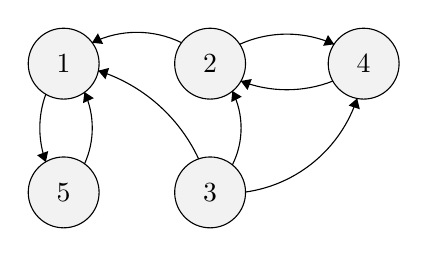
\begin{tikzpicture}[scale=0.15]
\tikzstyle{every node}+=[inner sep=0pt]
\draw [black,fill=gray!10] (20.5,-16.8) circle (3);
\draw (20.5,-16.8) node {$1$};
\draw [black,fill=gray!10] (32.9,-16.8) circle (3);
\draw (32.9,-16.8) node {$2$};
\draw [black,fill=gray!10] (32.9,-27.7) circle (3);
\draw (32.9,-27.7) node {$3$};
\draw [black,fill=gray!10] (20.5,-27.7) circle (3);
\draw (20.5,-27.7) node {$5$};
\draw [black,fill=gray!10] (45.9,-16.8) circle (3);
\draw (45.9,-16.8) node {$4$};
\draw [black] (22.26,-19.204) arc (24.50554:-24.50554:7.344);
\fill [black] (22.26,-19.2) -- (22.14,-20.14) -- (23.05,-19.72);
\draw [black] (18.991,-25.126) arc (-159.89496:-200.10504:8.366);
\fill [black] (18.99,-25.13) -- (19.19,-24.2) -- (18.25,-24.55);
\draw [black] (35.4,-15.163) arc (114.36079:65.63921:9.698);
\fill [black] (43.4,-15.16) -- (42.88,-14.38) -- (42.47,-15.29);
\draw [black] (43.297,-18.272) arc (-68.57465:-111.42535:10.668);
\fill [black] (35.5,-18.27) -- (36.07,-19.03) -- (36.43,-18.1);
\draw [black] (22.905,-15.032) arc (116.29055:63.70945:8.568);
\fill [black] (22.9,-15.03) -- (23.84,-15.13) -- (23.4,-14.23);
\draw [black] (23.434,-17.399) arc (72.36135:25.00562:14.084);
\fill [black] (23.43,-17.4) -- (24.04,-18.12) -- (24.35,-17.16);
\draw [black] (45.349,-19.741) arc (-17.99341:-82.04951:11.636);
\fill [black] (45.35,-19.74) -- (44.63,-20.35) -- (45.58,-20.66);
\draw [black] (34.776,-19.112) arc (26.7383:-26.7383:6.976);
\fill [black] (34.78,-19.11) -- (34.69,-20.05) -- (35.58,-19.6);
\end{tikzpicture}
\end{center}
Since $3 \to 1$ but $1 \not\to 3$, state 3 is transient. So state 1, 2, 4, and 5 are recurrent. The closed irreducible sets are $\{1,5\}$ and $\{2,4\}$.
\end{proof}

\item
???
\begin{proof}
The directed graph representation is
\begin{center}
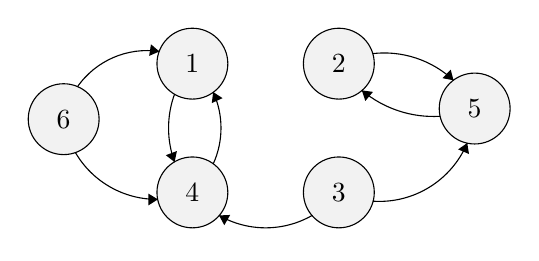
\begin{tikzpicture}[scale=0.15]
\tikzstyle{every node}+=[inner sep=0pt]
\draw [black,fill=gray!10] (20.5,-16.8) circle (3);
\draw (20.5,-16.8) node {$1$};
\draw [black,fill=gray!10] (32.9,-16.8) circle (3);
\draw (32.9,-16.8) node {$2$};
\draw [black,fill=gray!10] (32.9,-27.7) circle (3);
\draw (32.9,-27.7) node {$3$};
\draw [black,fill=gray!10] (20.5,-27.7) circle (3);
\draw (20.5,-27.7) node {$4$};
\draw [black,fill=gray!10] (44.4,-20.6) circle (3);
\draw (44.4,-20.6) node {$5$};
\draw [black,fill=gray!10] (9.6,-21.5) circle (3);
\draw (9.6,-21.5) node {$6$};
\draw [black] (22.26,-19.204) arc (24.50554:-24.50554:7.344);
\fill [black] (22.26,-19.2) -- (22.14,-20.14) -- (23.05,-19.72);
\draw [black] (18.991,-25.126) arc (-159.89496:-200.10504:8.366);
\fill [black] (18.99,-25.13) -- (19.19,-24.2) -- (18.25,-24.55);
\draw [black] (35.761,-15.949) arc (96.56235:46.86694:8.583);
\fill [black] (42.61,-18.21) -- (42.37,-17.3) -- (41.68,-18.03);
\draw [black] (41.485,-21.254) arc (-86.48313:-130.08758:9.406);
\fill [black] (34.85,-19.06) -- (35.14,-19.96) -- (35.79,-19.19);
\draw [black] (43.772,-23.516) arc (-22.79646:-93.82189:8.076);
\fill [black] (43.77,-23.52) -- (43,-24.06) -- (43.92,-24.45);
\draw [black] (10.766,-18.759) arc (145.01099:81.63971:7.195);
\fill [black] (17.71,-15.77) -- (16.99,-15.16) -- (16.84,-16.14);
\draw [black] (17.576,-28.289) arc (-89.38726:-149.87582:7.98);
\fill [black] (17.58,-28.29) -- (16.77,-27.8) -- (16.78,-28.8);
\draw [black] (30.642,-29.648) arc (-60.09093:-119.90907:7.906);
\fill [black] (22.76,-29.65) -- (23.2,-30.48) -- (23.7,-29.61);
\end{tikzpicture}
\end{center}

Since $3 \to 4$ but $4 \not\to 3$, state 3 is transient, and since $6 \to 1$ but $1 \not\to 6$, state 6 is transient. So state 1, 2, 4, and 5 are recurrent. The closed irreducible sets are $\{1,4\}$ and $\{2,5\}$.
\end{proof}

\end{enumerate}

\begin{prob}
Let $G$ be a connected graph. Let $X_n$ be a simple random walk on $G$. Show that the Markov chain $\{X_n\}$ is irreducible. (Hint: for any two vertices $x$ and $y$ in $G$, consider a path of consecutive nodes from $x$ to $y$.)
\end{prob}

\begin{proof}
Let $x$ and $y$ be any two vertices in $G$, let $T_y = \min\{n \geq 0 : X_n  =y\}$ be the first hitting time of $y$, and let $K$ be the smallest number of steps it takes to get from $x$ to $y$. Since $G$ is connected, $x$ and $y$ are connected by with a path of edges by definition, which implies that $p^K(x,y)>0$. So, for the the chain started in $x$, there exists a sequence $\{y_1, y_2, \dotsc, y_{K-1}\}$ such that 
\[
	p(x, y_1)>0, p(y_1,y_2)>0,\dotsc, p(y_{K-1},y_K)>0,
\] 
where $y_i \neq x$ for $i=1,2,\dotsc, K-1$. Then 
\[
	P_x(T_y < \infty) = p(x, y_1)p(y_1,y_2) \cdots p(y_{K-1},y_K)p(y_K,y) > 0.
\]
By the same logic, for the chain started in $y$, we see that $\{X_n\}$ on $G$ has exactly one communicating class, and hence is irreducible. 
\end{proof}

\begin{prob}
Let $G$ be a graph with two disjoint components $G_1$ and $G_2$. Let $X_n$ be a simple random walk on $G$.
\end{prob}

\begin{enumerate}
\item
Prove $\{X_n\}$ is not an irreducible Markov chain. 

\begin{proof}
Since $G_1 \cap G_2 = \emptyset$, there is no edge between any node in $G_1$ and any node in $G_2$, and hence $G_1$ and $G_2$ are disconnected. Then $\{X_n\}$ on $G$ is not irreducible. 
\par
If it were the case that $G_1$ and $G_2$ are connected, then there would exists a path between any two nodes $x_1, y_1 \in G_1$, i.e., $x_1 \leftrightarrow y_1$, and $x_2, y_2 \in G_2$, i.e., $x_2 \leftrightarrow y_2$. However, $G_1$ and $G_2$ are disconnected as previously noted, $x_1,y_1 \not\leftrightarrow x_2,y_2$. But $x_1 \leftrightarrow y_1$ and $x_2 \leftrightarrow y_2$. So, there exists two communicating classes, and hence $\{X_n\}$ on $G$ does not satisfy the definition of an irreducible Markov chain.
\end{proof}

\item
Let $P$ be the transition matrix of $X_n$. Let $P_1$ and $P_2$ be the transition matrices for the SRW on $G_1$ and $G_2$, respectively. Let $V_1 =\{1,\dotsc,k\}$ and $V_2 =\{k+1,\dotsc,k+l\}$ be the set of vertices in $G_1$ and $G_2$. Show that $P$ is of the following block diagonal form 
\begin{equation}\label{eq:block-diag}
	P = \begin{pmatrix}
		P_1 & 0 \\
		0 & P_2 
	\end{pmatrix}.
\end{equation}
Note a block diagonal matrix is a \emph{reducible} matrix.

\begin{proof}
We have $P(i,j) = 0$ for all $[i] \neq [j]$ since $V_1 \cap V_2 = \emptyset$. If $[i] = [j]$ and $i \in V_1$, then $X_n$ has transition matrix $P_1$, and if $i \in V_2$, $X_n$ has transition matrix $P_2$. Hence, $P$ is of the block diagonal form \eqref{eq:block-diag}.
\end{proof}


\item
Show the the SRW $\{X_n\}$ on $G$ has infinitely many stationary distributions. 

\begin{proof}
Since the disjoint graphs $G_1$ and $G_2$ are finite, $P_1$ has a stationary distribution, call it $\pi_1$, and $P_2$ has stationarity distribution, call it $\pi_2$. Note that $\pi_1$ has dimension $1\times k$, $\pi_2$ has dimension $1 \times l$. Let 
\[
	\pi = \begin{cases}
		(\pi_1, 0) & \text{if } X_0  \in G_1 \\
		(0, \pi_2) & \text{if } X_0  \in G_2 \\ 
	\end{cases}
\] 
be the stationary distribution for the operators $P$ on $G$, and note that $\pi$ has dimension $1 \times k+l$. Note also that $P$ has dimension $(k+l) \times (k+l)$. Now, for the chain started on any vertex in $G_1$, let $\pi = (\pi_1, 0)$ where $0$ is a $1 \times l$ dimensional vector. Then 
\[
	\begin{pmatrix}
		\pi_1 & 0
	\end{pmatrix}
	\begin{pmatrix}
		P_1 & 0 \\
		0 & P_2 
	\end{pmatrix} 
	= \begin{pmatrix} 
	\pi_1 P_1 & 0 
	\end{pmatrix}
	= \begin{pmatrix}
		\pi_1& 0
	\end{pmatrix},
\] 
where the last equality follows since $\pi_1$ was defined to be the stationary distribution for $P_1$. For the chain started on any vertex in $G_2$, $\pi =  (0,\pi_2)$ where here $0$ is a $1 \times k$ vector. So
\[
	\begin{pmatrix}
		0 & \pi_2
	\end{pmatrix}
	\begin{pmatrix}
		P_1 & 0 \\
		0 & P_2 
	\end{pmatrix} 
	= \begin{pmatrix}
		0 & \pi_2 P_2
	\end{pmatrix}
	= \begin{pmatrix}
		0 & \pi_2
	\end{pmatrix}
\]
For $0 \leq \lambda \leq 1$,
\[
	( \lambda \pi_1 + (1-\lambda) \pi_2 ) = ( \lambda \pi_1 P + (1-\lambda) \pi_2 P)
\]
is also stationary distribution for $P$ since of the block diagonal form \eqref{eq:block-diag}. Hence, there exists infinitely stationary for $X_n$ on $G$. 
\end{proof}
\end{enumerate}

\begin{prob}
Consider a Markov chain with state space $S=\{1,2\}$ and transition matrix 
\[
	P = \begin{pmatrix}
		1-a & a \\
		b & 1-b
	\end{pmatrix},
\]
where $0<a<1$ and $0<b<1$. 
\end{prob}

\begin{enumerate}
\item
Find its stationary distribution $\pi$. 
\begin{proof}
Let $\pi = (x,y)$. Then 
\[
	\pi P = \pi 
	\implies 
	\begin{cases}
		(1-a)x + by = x \\
		a x + (1-b)y = y
	\end{cases}
	\implies 
	ax = by. 
\]
Recalling that $x+y = 1$ gives the unique stationary distribution 
\[
	\pi = \left(\frac{b}{a+b},\frac{a}{a+b}\right).
\]
\end{proof}

\item
Use the Markov property to show that 
\[
	P(X_{n+1} = 1) - \frac{b}{a+b} = (1-a-b)\left[P(X_n = 1)- \frac{b}{a+b}\right].
\]

\begin{proof}
Start from the left hand side and condition on $X_n$ to obtain 
\begin{align*}
	P(X_{n+1} = 1) &= \sum_i  P(X_{n+1} = 1 \mid X_n = i) P(X_n = i) \\
						    &= (1-a) P(X_n=1) + b[1-P(X_n=1)] \\
						    &= P(X_n = 1) - aP(X_n=1) + b - bP(X_n=1) \\
						    &= (1-a-b)P(X_n=1) + b \\
						    &= (1-a-b)P(X_n=1) + \frac{b(a+b)}{a+b} \\
						    &= (1-a-b)P(X_n=1) + \frac{ab}{a+b} + \frac{b^2}{a+b}.
\end{align*}
Next, subtract $b/(a+b)$ from both sides 
\[
	P(X_{n+1} = 1) -\frac{b}{a+b} = (1-a-b)P(X_n=1) + \frac{ab}{a+b} + \frac{b^2}{a+b} - \frac{b}{a+b}.
\]
Simplifying the above expression gives
\[
	P(X_{n+1} = 1) - \frac{b}{a+b} = (1-a-b)\left[P(X_n = 1)- \frac{b}{a+b}\right].
\]
\end{proof}

\item
Use mathematical induction to show that 
\[
	P(X_n = 1) = \frac{b}{a+b} + (1-a-b)^n \left[P(X_0 = 1)- \frac{b}{a+b}\right]
\]

\begin{proof}[Proof (by induction on $n$)]
The base case $n=0$ holds since 
\begin{align*}
	P(X_0 = 1) &= \frac{b}{a+b} + (1-a-b)^0 \left[P(X_0 = 1)- \frac{b}{a+b}\right] \\
					 &= \frac{b}{a+b} + P(X_0 = 1)- \frac{b}{a+b} = P(X_0 = 1),
\end{align*} 
and the base case $n=1$ holds since
\begin{align*}
	P(X_1 = 1) &= \sum_{i} P(X_{1} = 1 \mid X_0 = i) P(X_0 = i) \\
					&= P(X_{1} = 1 \mid X_0 = 1) P(X_0 = 1) +  P(X_{1} = 1 \mid X_0 = 2) P(X_0 = 2) \\
					&= (1-a) P(X_0 = 1) +  b (1- P(X_0 = 1) )\\
					&=\frac{b}{a+b} + (1-a-b) \left[P(X_0 = 1)- \frac{b}{a+b}\right]
\end{align*}
where the last equality uses the same logic as in $(ii)$.
\par
Assume the claim is true for any $n$. We want to show that the result is also true for $n+1$. From (i), we know that 
\[
	P(X_{n+1} = 1) = \frac{b}{a+b} + (1-a-b)\left[P(X_n = 1)- \frac{b}{a+b}\right].
\]
Substituting in for $P(X_n=1)$ gives 
\begin{align*}
	P(X_{n+1} = 1) &= \frac{b}{a+b} + (1-a-b)\left[\left[(1-a-b)^n \left[P(X_0 = 1)- \frac{b}{a+b}\right]\right] - \frac{b}{a+b}\right] \\
	&= \frac{b}{a+b} + (1-a-b)^{n+1}\left[P(X_0 = 1)- \frac{b}{a+b}\right].
\end{align*}	
Shifting the indices back one period gives
\[
	P(X_n = 1) = \frac{b}{a+b} + (1-a-b)^n \left[P(X_0 = 1)- \frac{b}{a+b}\right].
\]
\end{proof}

\item
Show that $P(X_n=1)$ converges exponentially fast to $\pi(1)$ for the $\pi$ you found in (i).

\begin{proof}
Since $0<a<1$ and $0<b<1$, the term $|1-a-b| < 1$. Then, noting that $(1-a-b)^n$ is the only term depending on $n$, we have
\begin{align*}
	\lim_{n \to \infty} P(X_n = 1) &= \lim_{n \to \infty}\left[ \frac{b}{a+b} + (1-a-b)^n \left[P(X_0 = 1)- \frac{b}{a+b}\right]\right] \\
	&=  \frac{b}{a+b} + \lim_{n \to \infty} (1-a-b)^n  \left[ P(X_0 = 1) - \frac{b}{a+b} \right] \\	
		&=  \frac{b}{a+b} + O((1-a-b)^{n}). 
\end{align*}
That is, convergence to the limiting distribution, $P(X_n=1) \to \pi(1)$ as $n \to \infty$, is exponentially fast
\end{proof}
\end{enumerate}



\end{document}
